\documentclass[11pt,a4paper]{article}

\usepackage[margin=2.5cm]{geometry}
\usepackage{graphicx}
\usepackage{booktabs}
\usepackage{amsmath}
\usepackage{amssymb}
\usepackage{microtype}
\usepackage{xcolor}
\usepackage[colorlinks=true,linkcolor=black,
            citecolor=black,urlcolor=blue]{hyperref}
\usepackage{enumitem}
\usepackage{bm}
\usepackage[numbers,sort&compress]{natbib}
% ---- Macros generated by paper_analysis.py ---------------------------------
% Auto-generated by paper_analysis.py
\newcommand{\NcellsDiss}{9}
\newcommand{\NRegimes}{6}
\newcommand{\NTargets}{4}
\newcommand{\Npop}{200}
\newcommand{\Nalleles}{4}
\newcommand{\Tmax}{50}
\newcommand{\Tobs}{20}
\newcommand{\MutRate}{0.005}
\newcommand{\SelCoeff}{0.05}
\newcommand{\RidgeAlpha}{1.0}
\newcommand{\CVFolds}{5}
\newcommand{\FreqDepAlpha}{0.5}
\newcommand{\EcoK}{1.0}
\newcommand{\EcoRgrowth}{0.3}
\newcommand{\NGroups}{10}
\newcommand{\GroupSize}{20}
\newcommand{\SWithin}{0.05}
\newcommand{\SBetween}{0.08}
\newcommand{\Nreps}{100000}
\newcommand{\Nintervs}{100000}
\newcommand{\DeltaGene}{0.10}
\newcommand{\DeltaLin}{0.02}
\newcommand{\AlleleTol}{0.05}
\newcommand{\FlagPredScore}{0.483}
\newcommand{\FlagPredLo}{0.473}
\newcommand{\FlagPredHi}{0.491}
\newcommand{\FlagCausGap}{-0.008}
\newcommand{\FlagCausLo}{-0.009}
\newcommand{\FlagCausHi}{-0.008}
\newcommand{\FdCausGap}{-0.006}
\newcommand{\GrpPredScore}{0.371}
\newcommand{\GrpCausGap}{+0.112}


% ── Notation shorthands ──────────────────────────────────────────────────────
\newcommand{\Robs}{t_0}
\newcommand{\Tfin}{T_{\max}}
\newcommand{\DeltaY}{\Delta\bar{y}}
\newcommand{\lev}[1]{\textit{#1}}

\title{Predictive and causal access dissociate across\\
       levels of biological organization}

\author{Kunal Bhatia\\
\small Independent Researcher, Heidelberg\\
\small \texttt{kunal29bhatia@gmail.com}}

\date{March 2026\quad\textit{Preprint --- not peer reviewed}}

\begin{document}
\maketitle
\vspace{-6pt}

% ── Abstract ─────────────────────────────────────────────────────────────────
\begin{abstract}
\noindent
Which level of biological organization gives the best forecast of evolutionary
change?
Which gives the most reliable handle for intervention?
We argue these questions have different answers.
Using a simulation study spanning six evolutionary regimes---random genetic drift,
directional selection, Moran dynamics, frequency-dependent selection,
eco-evolutionary feedback, and group-structured selection---we evaluate four
biologically motivated description levels (gene composition, lineage composition,
organism-level fitness, and an organism-plus-ecology summary) as predictors
of four evolutionary targets, and four level-targeted interventions for
their causal effects on the same targets.
We identify \NcellsDiss{} dissociation cells in which the level achieving the
highest cross-validated predictive score differs from the level whose targeted
perturbation produces the largest causal effect on the same outcome.
The clearest mechanistic case is eco-evolutionary feedback on the resource target:
the organism-plus-ecology summary achieves $R^2 = \FlagPredScore{}$
[\FlagPredLo{}, \FlagPredHi{}] for future resource state, yet a gene-level
intervention is the only perturbation that reliably alters resource state,
and does so negatively (gap $= \FlagCausGap{}$ [\FlagCausLo{}, \FlagCausHi{}])
because the favored allele carries the highest per-capita consumption rate.
Across all \NcellsDiss{} dissociation cells, gene-level interventions dominate
causally while higher-level summaries dominate predictively.
We conclude that identifying the best-predicting level and identifying the
best-intervening level are distinct empirical questions, and both are necessary
for a complete account of multilevel evolutionary dynamics.
\end{abstract}

\bigskip
\noindent\textbf{Keywords:}\enspace
multilevel selection; eco-evolutionary dynamics; causal inference; levels of organization;
genotype--phenotype mapping; prediction versus intervention; evolutionary forecasting

\clearpage

% ── Introduction ──────────────────────────────────────────────────────────────
\section{Introduction}
\label{sec:intro}

Evolution can be described at multiple levels of biological organization,
and for many purposes the choice of level is not arbitrary.
A gene-centric description~\citep{Dawkins1976, Williams1966} accounts precisely
for the heritable substrate on which natural selection acts, and has proven
indispensable for calculating allele-frequency trajectories in large populations
under known fitness parameters~\citep{Fisher1930, Wright1931, Crow1970}.
A phenotype- or organism-level description captures the expression of genetic
variation in fitness-relevant traits and is the natural unit for quantitative
genetics~\citep{Falconer1996, Lynch1998, Lande1979}.
Group- and community-level descriptions are required when fitness consequences
operate between groups or when ecological partners co-evolve on
comparable timescales~\citep{Wilson1975, Hamilton1964, Nowak2006,
Post2009, Pelletier2009, Schoener2011}.
Multilevel selection theory formalises the conditions under which each level
contributes net selection~\citep{Price1970, Hamilton1975, Frank1995,
Okasha2006, Kerr2002}, but it does not directly address which level offers
the best empirical forecast of near-term evolutionary outcomes.

Forecasting is a distinct problem.
Population-genetic models can predict allele-frequency trajectories in simple
selection regimes, but empirical prediction of evolutionary change in complex
systems is uncertain~\citep{Barton2002, Orr2009, Nosil2017}.
Phenotypic summaries often achieve better empirical forecast accuracy than
allele-level summaries when allele effects are small, numerous, or
pleiotropic~\citep{Meuwissen2001, Goddard2010, Wray2013}.
Ecology adds another layer: when gene frequencies feed back into ecological
state and vice versa, no single level naturally encompasses the whole
dynamical system~\citep{Hairston2005, Yoshida2003, Ellner2011, Hendry2016}.

Intervention is yet another distinct problem.
Identifying which level best forecasts an outcome does not imply that intervening
at that level will produce the largest or most reliable change in that outcome.
A description level achieves predictive power by encoding relevant information---it
may do so by compressing variation that is already causally upstream.
Causal power, in the sense of a successful targeted intervention~\citep{Pearl2009,
Woodward2003, Spirtes2000}, requires that the intervened variable be in the
generative architecture of the outcome.
These two properties---informational compression and causal position---can,
in principle, be held by different levels simultaneously.

This distinction has been noted in several specific contexts.
In quantitative genetics, selection response can be predicted from population-mean
phenotype, but realized change depends on allelic architecture and linkage
disequilibrium~\citep{Turelli1994, Hansen2006, deVladar2011}.
In eco-evolutionary dynamics, aggregate population state can track ecological
conditions well, but evolutionary change is ultimately driven by allele
sorting~\citep{Ellner2011, Pelletier2009, Hairston2005}.
In group-selection models, group fitness differentials contribute a predictable
component to allele spread, but allele composition remains the mechanistic
substrate~\citep{Price1970, Okasha2006, West2007}.
What is lacking is a systematic, cross-regime test that measures both predictive
access and causal access at multiple levels simultaneously, with the two
quantities assessed against the same outcome target.

Here we provide such a test.
We implement six evolutionary regimes in a controlled simulation and measure,
for each regime and each outcome target, (i) the best description level for
predicting the target (\emph{predictive access}, assessed by a cross-validated
predictive score: $R^2$ for continuous targets and AUC for dominance) and (ii) the description level whose targeted perturbation produces
the largest reliable change in that target (\emph{causal access}, assessed
by mean intervention--control gap with bootstrap confidence intervals).
We find that the two measures dissociate in \NcellsDiss{} (regime, target)
cells, and that the pattern of dissociation is mechanistically interpretable
in each case.

The paper is organized as follows.
Section~\ref{sec:methods} describes the model, observer definitions, targets,
and scoring procedures.
Section~\ref{sec:results} presents the main results in four subsections:
the flagship eco-evolutionary case (Section~\ref{sec:flagship}),
the full dissociation pattern (Section~\ref{sec:dissociation}),
regime-wide predictive and causal maps (Section~\ref{sec:maps}),
and the neutral drift control (Section~\ref{sec:neutral}).
Section~\ref{sec:discussion} interprets the results in terms of multilevel
selection theory, eco-evolutionary dynamics, and the general prediction--intervention
distinction.

% ── Methods ───────────────────────────────────────────────────────────────────
\section{Model and scoring framework}
\label{sec:methods}

\subsection{Population model}

We simulate a haploid asexual population of $N = \Npop$ individuals,
each carrying one of $K = \Nalleles$ alleles.
Allele identity can change by mutation at rate $\mu = \MutRate$ per individual
per generation; allele $i$ mutates to allele $j$ drawn uniformly from all $K$
alleles (including $i$).
In addition to allele identity, every individual carries a \emph{lineage tag}
equal to its founder's index at $t = 0$.
Lineage tags are never altered by mutation; they propagate by clonal inheritance
and track the coalescent history of the population independently of allele
composition.

Populations are initialized with alleles drawn uniformly from $\{0,\ldots,K-1\}$.
Each replicate is run for $\Tfin = \Tmax$ generations.
A snapshot is recorded at $t = \Robs = \Tobs$ (the \emph{observation horizon})
and at $t = \Tfin$ (the \emph{prediction horizon}).
The observation-horizon snapshot is used to form observer features;
the prediction-horizon snapshot defines targets.

\subsection{Evolutionary regimes}
\label{sec:regimes}

Six evolutionary regimes are implemented.

\subsubsection{Random genetic drift.}
Fitness $w_i = 1$ for all individuals.
Reproduction follows the Wright--Fisher model:
offspring are sampled with replacement proportional to fitness (uniform).
All changes in composition are due to sampling variance.

\subsubsection{Directional selection.}
The favored allele (allele 0) has fitness $w_0 = 1 + s$, $s = \SelCoeff$;
all others have $w = 1$.
Reproduction is Wright--Fisher.

\subsubsection{Moran selection dynamics.}
Same directional fitness scheme as above.
Dynamics are birth--death: each timestep, one individual is chosen for
reproduction proportional to fitness, one is chosen for death uniformly;
$N$ such steps constitute one generation.
Moran dynamics yield slower allele-frequency change than Wright--Fisher
sampling~\citep{Moran1958, Nowak2006}.

\subsubsection{Frequency-dependent selection.}
Fitness of allele $a$ decreases with its own frequency:
$w_a(t) = 1 - \alpha\,p_a(t)$, $\alpha = \FreqDepAlpha$.
This implements a simple negative frequency-dependent selection scheme,
maintaining allele diversity by disfavoring common types---a minimal
analogue of models for balancing selection and
niche partitioning~\citep{Ayala1974, Charlesworth2006, Delph2016}.

\subsubsection{Eco-evolutionary feedback.}
Fitness is resource-dependent:
$w_a(t) = b_a\,R(t)/K$,
where $b_a \in \{1.16, 1.10, 1.04, 0.98\}$ for alleles $0$--$3$,
$K = \EcoK$ is the resource carrying capacity, and $R(t)$ follows
logistic growth with consumption:
\begin{equation}
  R(t+1) = R(t) + r_R R(t)\!\left(1 - \frac{R(t)}{K}\right)
              - \bar{c}(t)\,\frac{R(t)}{K},
  \label{eq:eco}
\end{equation}
where $r_R = \EcoRgrowth$, and $\bar{c}(t) = \sum_a p_a(t)\,c_a$ is the
mean per-capita consumption rate with
$c_a \in \{0.20, 0.15, 0.10, 0.05\}$.
Allele 0, which is favored by highest base fitness, also has the highest
per-capita consumption rate.
This coupling---favored allele depletes the shared resource---is the structural
source of the flagship dissociation.
Eco-evolutionary feedback of this form has been studied extensively
in natural~\citep{Yoshida2003, Hairston2005, Schoener2011} and theoretical
contexts~\citep{Post2009, Ellner2011, Hendry2016}.

\subsubsection{Group-structured selection.}
$N = \NGroups \times \GroupSize$ individuals are partitioned into
$\NGroups$ groups of $\GroupSize$.
Each generation: (i) within-group Wright--Fisher sampling with directional
selection coefficient $s_\mathrm{within} = \SWithin$;
(ii) one between-group event, in which a reproducing group is selected
proportional to group mean fitness (with between-group advantage
$s_\mathrm{between} = \SBetween$) and replicates into a randomly chosen group.
This implements a two-level selection structure following
\citet{Wilson1975} and formalized by \citet{Price1970}.

\subsection{Description levels (observers)}
\label{sec:observers}

Four biologically motivated description levels are evaluated at $t_0$:

\paragraph{Gene composition.}
The allele frequency vector $\bm{p}(t_0) \in \mathbb{R}^K$.
This is the minimal sufficient statistic for allelic state and is the
upstream node in the generative architecture of every regime.
It carries no information about fitness unless the genotype--fitness
map is known~\citep{Falconer1996, Fisher1930}.

\paragraph{Lineage composition.}
A permutation-invariant summary of the founder-lineage frequency
spectrum: the sorted top-20 lineage frequencies, the number of surviving
lineages, lineage entropy, and maximum lineage share.
This captures coalescent structure and integrates the cumulative selective
history since founding~\citep{Kingman1982, Tajima1983}.

\paragraph{Organism-level fitness summary.}
A permutation-invariant summary of the realized fitness distribution at $t_0$:
20 quantiles, mean, variance, and the 10 highest individual fitness values.
Realized fitness is genotype-times-environment; two individuals with the
same allele may have different realized fitness values (e.g.,
in the eco-evolutionary regime where fitness depends on $R(t)$).

\paragraph{Organism\,+\,ecology summary.}
The organism-level fitness summary augmented by the current resource
value $R(t_0)$.
This level is informative about the ecological state of the system and
is meaningful only when resource dynamics are present.

\subsection{Evolutionary targets}
\label{sec:targets}

Four targets are measured at $t = \Tfin$:

\paragraph{Allele transmission.}
The frequency of the favored allele (allele 0) at $\Tfin$.
A continuous measure of fixation progress relevant to all selection regimes.

\paragraph{Allele dominance.}
A binary indicator for whether the favored allele (allele 0) exceeds
50\,\% frequency at $\Tfin$.
This target captures majority takeover rather than continuous fixation
progress and is scored by AUC in the predictive analysis.

\paragraph{Lineage persistence.}
The fraction of lineages with frequency $\geq 0.01$ at $t_0$ that
still have positive frequency at $\Tfin$.
A continuous measure of genetic diversity retention.

\paragraph{Resource level.}
$R(\Tfin)$; meaningful only in the eco-evolutionary regime.

\subsection{Predictive scoring}
\label{sec:pred}

For each (regime, target, observer) triple we generate $n = \Nreps$ independent
replicates.
Each replicate contributes observer features $\bm{x} = \phi(s_{t_0})$
and scalar target $y$.
Predictive access is measured by $K = \CVFolds$-fold cross-validated $R^2$
using ridge regression ($\alpha = \RidgeAlpha$, standardized inputs)
for continuous targets; AUC from logistic regression for binary targets
(allele dominance).
Confidence intervals are from $10^3$ bootstrap resamples of per-fold scores.
\emph{Confirmed} predictive access requires $\mathrm{CI}_\mathrm{lo} > 0$.

\subsection{Causal scoring}
\label{sec:caus}

For causal scoring we run $n = \Nintervs$ matched pairs per
(regime, target, intervention) triple.
Each pair: a control arm (no perturbation, $t_0 \to \Tfin$) and an
intervention arm (perturb at $t_0$, then evolve to $\Tfin$).
The \emph{causal gap} is $\DeltaY = \bar{y}_\mathrm{int} - \bar{y}_\mathrm{ctrl}$
with 95\,\% bootstrap CI.

Four intervention classes are defined, each population-size preserving:
\begin{enumerate}[label=\arabic*.,leftmargin=1.8em,itemsep=2pt]
  \item \textbf{Gene.} Shift mass $\delta = \DeltaGene$ from the most common
        non-favored allele to allele 0, by resampling $\lfloor\delta N\rfloor$
        individuals.
  \item \textbf{Lineage.} Redistribute mass $\delta_L = \DeltaLin$ from the
        most common lineage to the rarest surviving lineage.
        Arms in which the allele-composition shift exceeds $\AlleleTol$
        are classified \textsc{allele\_contaminated} and excluded.
  \item \textbf{Organism.} Increase the realized fitness of the bottom 10\,\%
        of individuals by $\delta$.
  \item \textbf{Ecology.} Perturb $R(t_0)$ by $+\delta$, clipped to $[0,2K]$.
\end{enumerate}
Causal comparisons are always within a fixed target; cross-target causal
comparisons are forbidden by design.

\subsection{Dissociation criterion}
\label{sec:diss}

A (regime, target) cell is a \emph{confirmed dissociation} if:
(i) at least one observer achieves confirmed predictive access
    ($\mathrm{CI}_\mathrm{lo} > 0$);
(ii) the observer with the highest cross-validated score differs
     from the intervention with the largest absolute causal gap;
(iii) both the predictive CI and the causal gap CI exclude zero.

% ── Results ───────────────────────────────────────────────────────────────────
\section{Results}
\label{sec:results}

\subsection{Eco-evolutionary feedback: mechanistic dissociation}
\label{sec:flagship}

The clearest dissociation arises in eco-evolutionary feedback dynamics
with the resource target (Figure~\ref{fig:flagship}).

\paragraph{Predictive side.}
At $t_0 = \Tobs$, the organism-plus-ecology summary is the strongest
predictor of resource state at $\Tfin = \Tmax$,
achieving $R^2 = \FlagPredScore{}$ [\FlagPredLo{}, \FlagPredHi{}]
(Figure~\ref{fig:flagship}A).
Gene composition is a substantially weaker predictor of the same quantity.
The mechanism is transparent: the organism-plus-ecology summary includes
$R(t_0)$ directly, and $R(t_0)$ is strongly autocorrelated with $R(\Tfin)$
because the resource dynamics are slow relative to the $\Tmax - \Tobs$
interval.
The fitness distribution further compresses information about which alleles
are abundant (via the allele--fitness coupling), giving the organism-plus-ecology
observer an informational advantage over gene composition alone.

\paragraph{Causal side.}
Applying a gene-level perturbation produces the only reliable causal effect
on resource state, with a gap of $\FlagCausGap{}$ [\FlagCausLo{}, \FlagCausHi{}]
(Figure~\ref{fig:flagship}B).
The sign is negative: increasing allele 0 frequency depletes the resource.
This is a direct consequence of Equation~\eqref{eq:eco}: allele 0 carries
the highest per-capita consumption rate ($c_0 = 0.20$) alongside the
highest base fitness ($b_0 = 1.16$).
Selective advantage and resource consumption are therefore positively
correlated; elevating allele 0 frequency increases mean consumption,
accelerating resource depletion.

Ecology and organism interventions are ineffective: their causal gaps
do not exclude zero.
This is expected because neither perturbation reaches the allele frequencies
that determine per-capita consumption.
The resource level responds to allele composition---not to fitness or ecology
shifts at $t_0$---because allele frequencies are the upstream node in the
feedback loop.

This cell is the most direct illustration of the general pattern.
High predictive accuracy comes from informational compression of autocorrelated
state; causal access requires reaching the upstream generative variable.
Both properties are present in the system, but they reside at different levels.

\begin{figure}[ht]
\centering
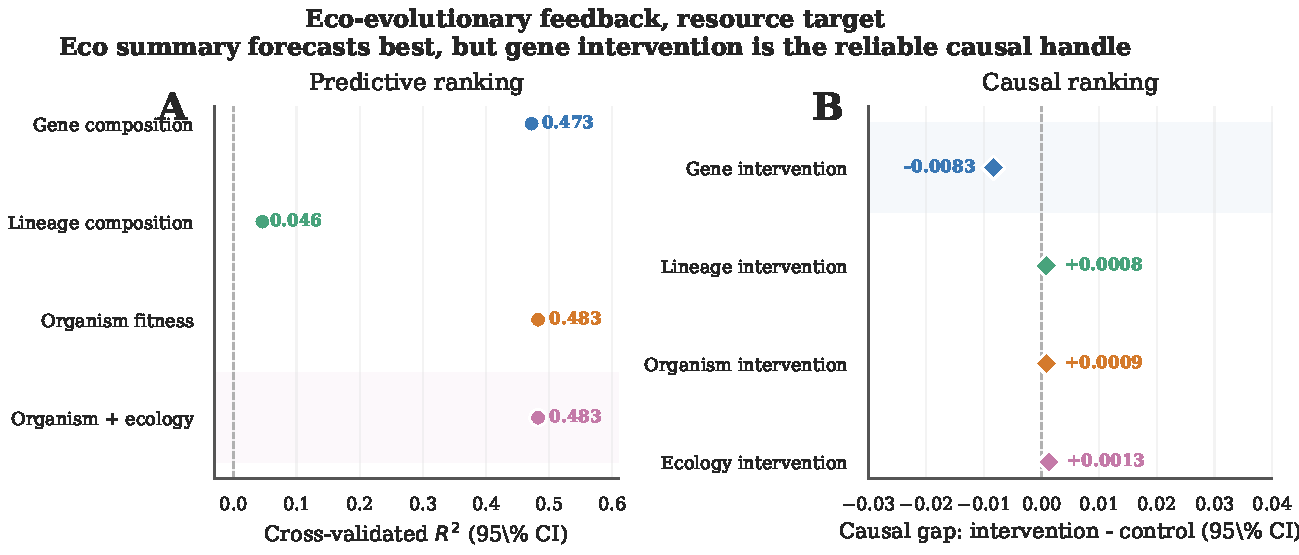
\includegraphics[width=0.90\textwidth]{outputs/figures/fig2_flagship.pdf}
\caption{\textbf{Eco-evolutionary feedback regime, resource target.}
\textbf{(A)} Cross-validated $R^2$ for each observer level at $t_0 = \Tobs{}$
predicting resource state at $\Tfin = \Tmax{}$ (dot = mean; bar = 95\,\% CI).
The organism-plus-ecology summary achieves $R^2 = \FlagPredScore{}$,
strongly outperforming gene composition.
\textbf{(B)} Causal gaps (intervention minus control; diamond = mean; bar = 95\,\% CI)
for each intervention class.
Gene intervention is the only perturbation that reliably changes resource state,
and does so negatively: the favored allele has the highest per-capita consumption rate.
Organism and ecology interventions do not reach the generative variable (allele frequencies).}
\label{fig:flagship}
\end{figure}

\subsection{Confirmed dissociation pattern}
\label{sec:dissociation}

Across all six regimes and four targets, we identify \NcellsDiss{} cells
satisfying the dissociation criterion (Table~\ref{tab:dissociation};
Figure~\ref{fig:dissociation}).
In all \NcellsDiss{} cells, gene composition is the causal winner.
In all \NcellsDiss{} cells, a higher-level summary is the predictive winner.

\begin{table}[t]
\centering
\caption{\textbf{Confirmed dissociation cells (n=\NcellsDiss{}).}
Predictive score is cross-validated $R^2$ for continuous targets and AUC for the
binary dominance target, each with 95\% bootstrap CI. Causal gap is intervention
minus control mean difference with 95\% CI.}
\label{tab:dissociation}
\footnotesize
\setlength{\tabcolsep}{4pt}
\resizebox{\textwidth}{!}{%
\begin{tabular}{llcccc}
\toprule
Regime & Target & Predictive winner & Predictive score & Causal winner & Causal gap (95\% CI) \\
\midrule
Group-structured selection & Allele transmission & Organism & $R^2$: $0.371$ [0.367, 0.375] & Gene & $+0.112$ [+0.110, +0.115] \\
Moran selection dynamics & Allele transmission & Organism & $R^2$: $0.463$ [0.459, 0.466] & Gene & $+0.094$ [+0.091, +0.096] \\
Directional selection & Allele dominance & Organism & AUC: $0.849$ [0.845, 0.852] & Gene & $+0.084$ [+0.081, +0.087] \\
Directional selection & Allele transmission & Organism & $R^2$: $0.423$ [0.419, 0.426] & Gene & $+0.068$ [+0.067, +0.070] \\
Eco-evolutionary feedback & Allele transmission & Org.+Eco. & $R^2$: $0.323$ [0.313, 0.332] & Gene & $+0.035$ [+0.034, +0.036] \\
Eco-evolutionary feedback & Lineage persistence & Lineage & $R^2$: $0.178$ [0.176, 0.179] & Gene & $+0.019$ [+0.019, +0.020] \\
Eco-evolutionary feedback & Resource level & Org.+Eco. & $R^2$: $0.483$ [0.473, 0.491] & Gene & $-0.008$ [-0.009, -0.008] \\
Directional selection & Lineage persistence & Lineage & $R^2$: $0.142$ [0.139, 0.145] & Gene & $+0.007$ [+0.006, +0.008] \\
Frequency-dependent selection & Lineage persistence & Lineage & $R^2$: $0.172$ [0.170, 0.174] & Gene & $-0.006$ [-0.007, -0.005] \\
\bottomrule
\end{tabular}%
}

\end{table}

\paragraph{Directional selection and Moran dynamics.}
Both regimes show dissociation on the transmission target.
Organism-level or organism-plus-ecology summaries outpredict gene composition:
at $t_0 = \Tobs$, the fitness distribution already encodes allele-sorting
progress via the allele--fitness coupling, so the organism observer achieves
predictive accuracy without directly measuring allele frequencies.
Yet gene interventions produce the largest causal gap on transmission.
The Moran regime shows the largest single causal gap,
consistent with its birth--death structure: each Moran step directly
replaces allele identity, so allele-frequency perturbations propagate
efficiently.

\paragraph{Frequency-dependent selection.}
The only cell in which lineage composition, rather than an organism or
organism-plus-ecology summary, is the predictive winner.
Under balancing selection, allele frequencies are held near their equilibrium
values, reducing the predictive information in gene composition for the
persistence target.
Lineage composition captures how diversity is distributed across founders,
which is strongly predictive of how much lineage diversity will persist.
Gene intervention still dominates causally (\FdCausGap{}):
shifting allele 0 frequency changes the negative frequency-dependent pressure
on rare alleles, which alters the selective forces maintaining lineage diversity.

\paragraph{Group-structured selection.}
Organism-level summary outpredicts gene composition on transmission
(\GrpPredScore{} vs.\ lower gene-level scores).
Between-group selection creates group-level fitness variance that the organism
observer captures via the fitness distribution, without requiring the observer
to track allele identity directly.
This is the cleanest example of the group-selection intuition in our
data: higher-level properties predict individual-level outcomes,
but the causal substrate remains allele composition (\GrpCausGap{}).

\begin{figure}[ht]
\centering
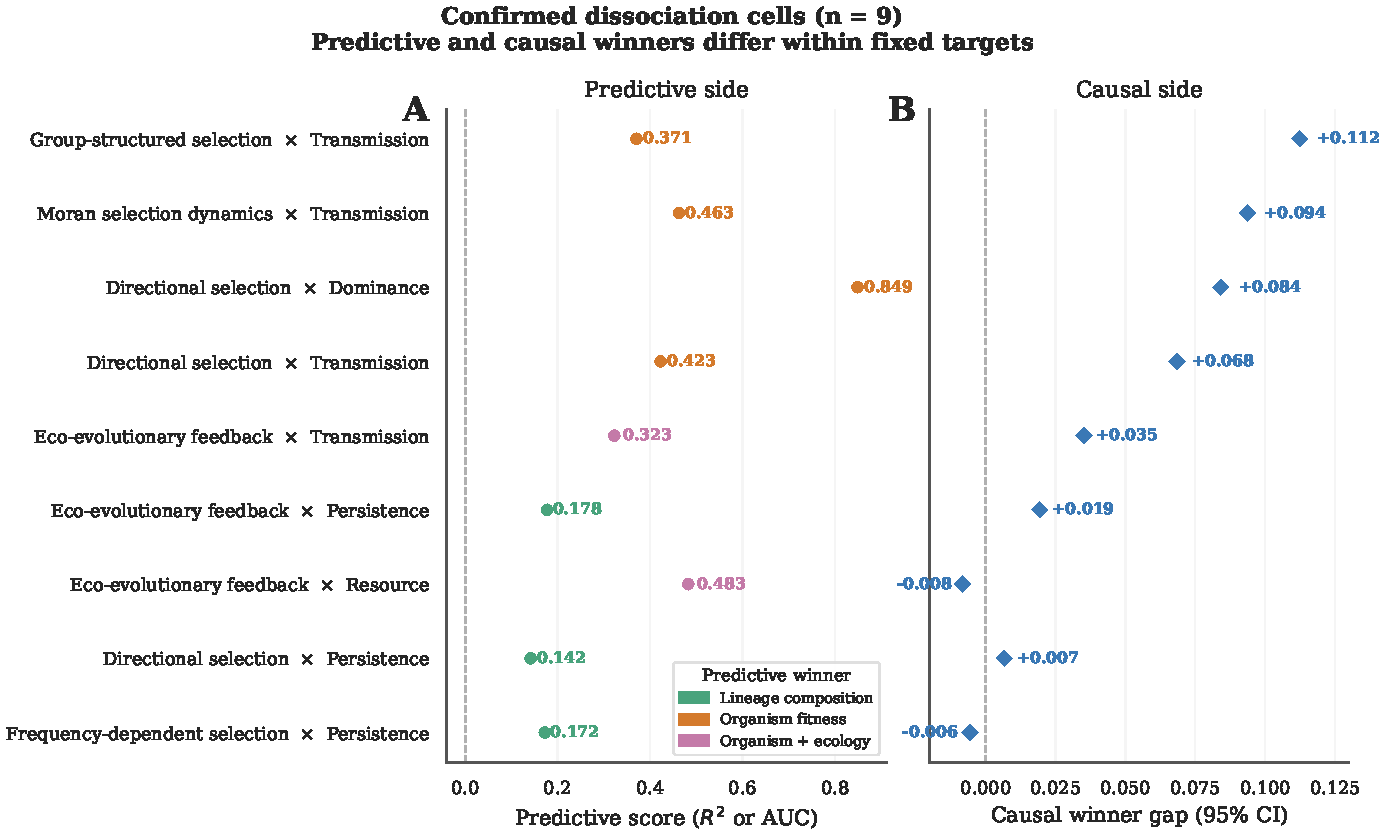
\includegraphics[width=0.88\textwidth]{outputs/figures/fig3_dissociation.pdf}
\caption{\textbf{Confirmed dissociation cells (n=\NcellsDiss{}).}
\textbf{(A)} Predictive winner score (cross-validated $R^2$ for continuous targets,
AUC for dominance; 95\,\% CI) for each cell. Color indicates winning observer level.
\textbf{(B)} Causal gap of the winning intervention (95\,\% CI) for each cell.
Gene composition is the causal winner in all \NcellsDiss{} cells;
a higher-level summary is the predictive winner in all \NcellsDiss{} cells.}
\label{fig:dissociation}
\end{figure}

\subsection{Regime-wide maps of predictive and causal access}
\label{sec:maps}

Figures~\ref{fig:pred_map} and \ref{fig:caus_map} show winner heatmaps
across all regime--target combinations.

\paragraph{Predictive map (Figure~\ref{fig:pred_map}).}
Gene composition is the predictive winner under random drift (via
temporal autocorrelation; Section~\ref{sec:neutral}) and achieves
moderate predictive power in directional and Moran regimes where
fitness differences are smallest.
The organism-plus-ecology observer dominates in the eco-evolutionary
regime for all targets, because $R(t_0)$ is the single strongest
autocorrelated predictor of near-term dynamics in that regime.
Lineage composition wins only under frequency-dependent selection
on the persistence target, consistent with the mechanism described above.

\paragraph{Causal map (Figure~\ref{fig:caus_map}).}
Gene interventions produce the largest confirmed causal gap in almost
every selection-driven cell for which a causal winner can be identified.
The uniformity of this pattern across regimes is strong evidence that
gene composition sits at the upstream causal node across all the
mechanisms studied, which is expected on theoretical grounds~\citep{Fisher1930,
Price1970, Frank1995}: heritable variation is allele-level variation, and
selection on allele frequencies is the generative event common to all regimes.
Ecology interventions occasionally show small causal gaps in the eco-evolutionary
regime but do not exceed the gene intervention gap, confirming that allele
composition---not the current ecological state---is the operative causal node.

\begin{figure}[ht]
\centering
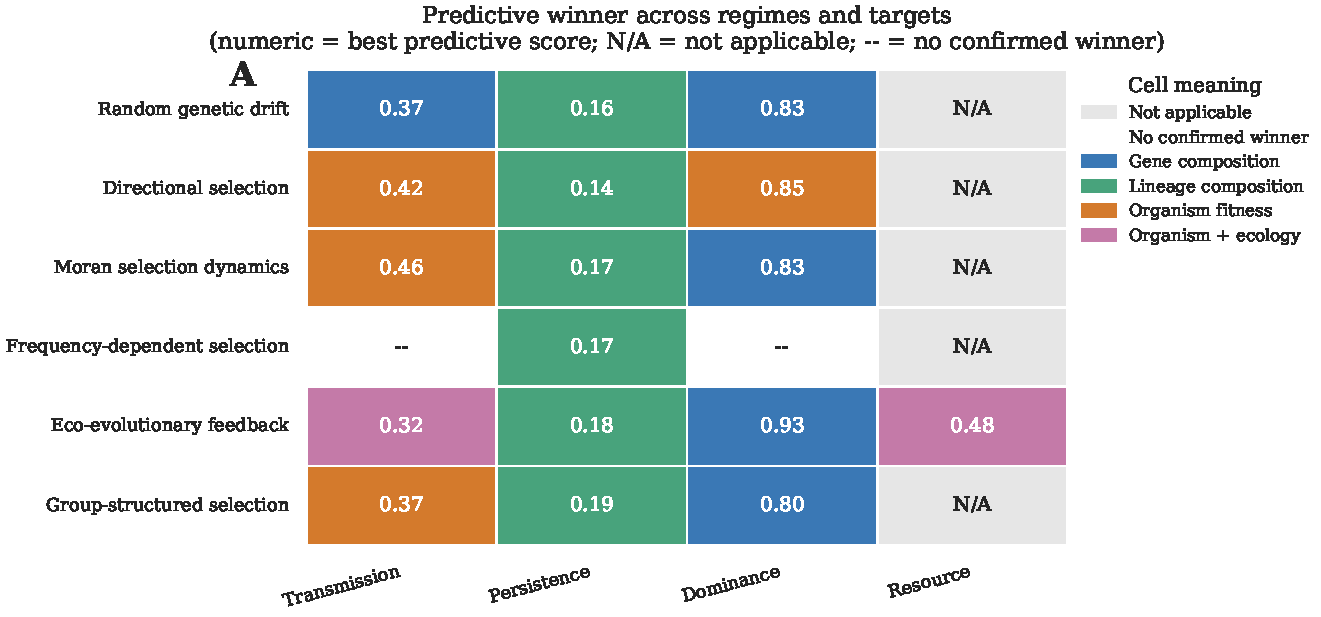
\includegraphics[width=0.76\textwidth]{outputs/figures/fig4_pred_map.pdf}
\caption{\textbf{Predictive winner map.}
Cell color indicates the winning observer level; cell value is the best
cross-validated score ($R^2$ for continuous targets, AUC for dominance).
Dashes indicate no confirmed predictive access ($\mathrm{CI_{lo}} \leq 0$)
or targets not applicable in that regime.}
\label{fig:pred_map}
\end{figure}

\begin{figure}[ht]
\centering
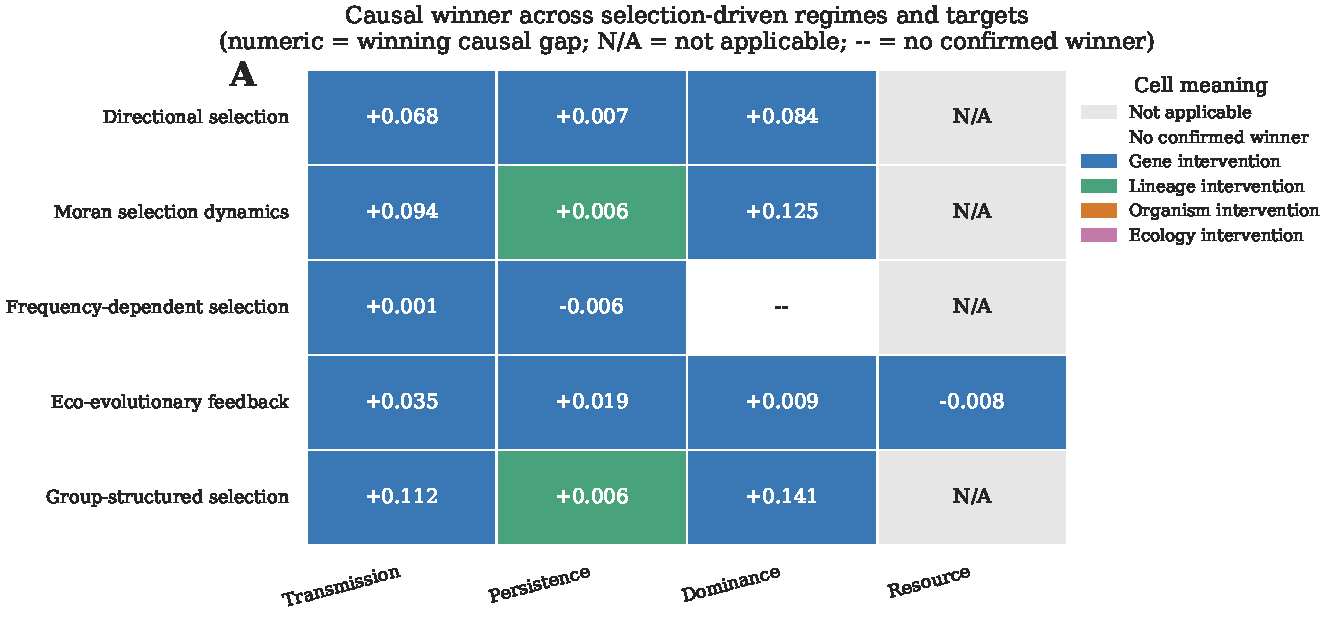
\includegraphics[width=0.74\textwidth]{outputs/figures/fig5_caus_map.pdf}
\caption{\textbf{Causal winner map.}
Cell color indicates the winning intervention level; cell value is the
winning causal gap.
Only selection-driven regimes shown; random drift produces no selective
causal gap. Dashes indicate no confirmed causal gap ($\mathrm{CI}$ includes zero).}
\label{fig:caus_map}
\end{figure}

\subsection{Neutral drift: the autocorrelation baseline}
\label{sec:neutral}

Under random genetic drift, gene composition at $t_0$ is the strongest
predictor of gene composition at $\Tfin$ (Figure~\ref{fig:neutral}).
This is expected: allele frequencies are positively autocorrelated
over time even under pure drift, because the Markov chain
moves slowly relative to the observation window.
Crucially, no dissociation is present here: gene composition is also
the strongest causal handle under drift---a gene intervention moves allele
frequencies and therefore transmission directly, though the causal gap
reflects sampling variance rather than selective pressure and is therefore
excluded from the causal winner map (Figure~\ref{fig:caus_map}), which
reports only selection-driven regimes.

We include this result to make two methodological points explicit.
First, high predictive power at the gene level is not evidence of
selection or of any mechanistically informative coupling; it can arise
purely from autocorrelation.
Second, confirming dissociation requires that a \emph{different} level
wins predictively---strong gene-level prediction alone does not imply
dissociation.

\begin{figure}[ht]
\centering
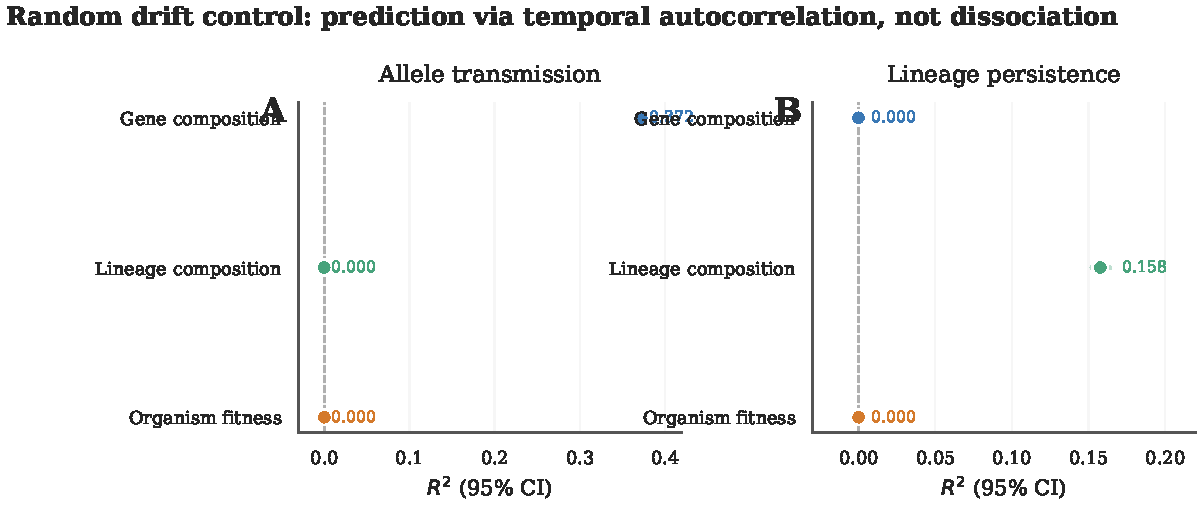
\includegraphics[width=0.72\textwidth]{outputs/figures/fig6_neutral.pdf}
\caption{\textbf{Random genetic drift: no dissociation.}
\textbf{(A)} Predictive scores, transmission target.
\textbf{(B)} Predictive scores, persistence target.
Gene composition achieves the highest predictive score via temporal
autocorrelation. Gene composition is also the causal winner under drift;
the dissociation criterion is not satisfied.}
\label{fig:neutral}
\end{figure}

\subsection{Boundary cells}
\label{sec:boundary}

Figure~\ref{fig:boundary} shows four cells in which the dissociation
criterion was not satisfied: eco-evolutionary feedback $\times$ dominance,
Moran selection dynamics $\times$ dominance, group-structured selection
$\times$ dominance, and group-structured selection $\times$ persistence.
In the three dominance cells, predictive access is present, but the predictive
and causal winner pattern does not satisfy the confirmed dissociation criterion.
In the group-structured persistence cell, predictive access is weak and no
confirmed dissociation emerges at the present parameter settings.
These non-dissociation cells establish the scope of the result and exclude
the interpretation that dissociation is universal.

\begin{figure}[ht]
\centering
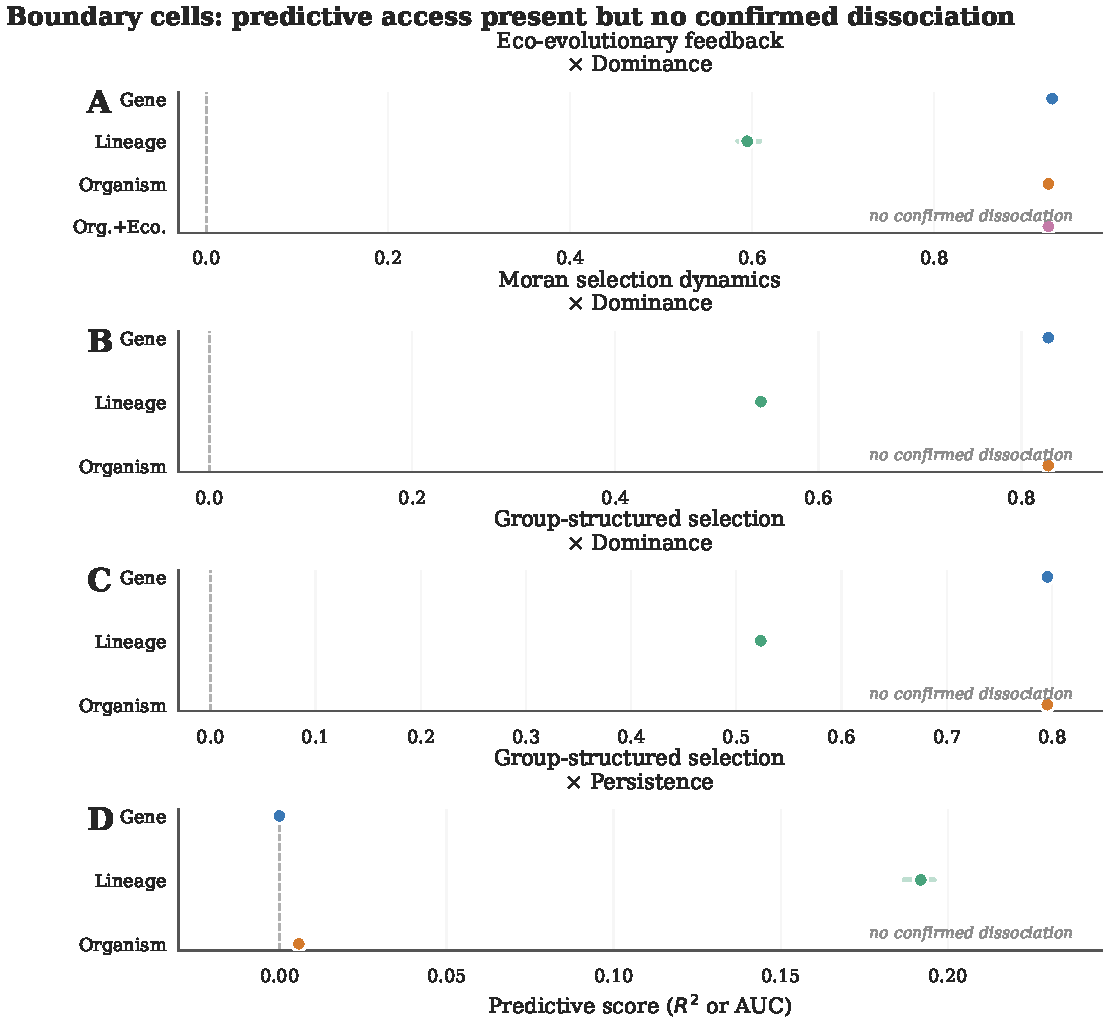
\includegraphics[width=0.78\textwidth]{outputs/figures/fig7_boundary.pdf}
\caption{\textbf{Boundary cells: no confirmed dissociation.}
Four cells examined for dissociation in which the criterion was not met:
either no observer achieved confirmed predictive access, or the predictive
and causal winners coincided.}
\label{fig:boundary}
\end{figure}

% ── Discussion ────────────────────────────────────────────────────────────────
\section{Discussion}
\label{sec:discussion}

\subsection{Prediction and causation as distinct empirical questions}

The central result is that the two activities most relevant to understanding
evolutionary change---forecasting and intervention---can require different
levels of biological description.
This is not a contradiction.
Predictive access is an epistemic property: it reflects the
mutual information between an observer and future state.
Causal access is a structural property: it reflects whether a
variable sits in the upstream part of the generative process.
These properties can be held, simultaneously, at different levels
of the same system.

The point has been noted informally in evolutionary biology for decades.
Quantitative geneticists have long observed that population-mean phenotype
predicts response to selection accurately in many settings~\citep{Lande1979,
Falconer1996}, while the actual allele-level changes are often poorly
tracked or not directly controlled~\citep{Barton2002, Charlesworth2010}.
The selective breeding community has empirically confirmed that genomic
prediction can outperform phenotype-based prediction in certain architectures,
yet the causal variants remain hard to identify and manipulate
directly~\citep{Meuwissen2001, Goddard2010, Hayes2009}.
Our results provide a controlled demonstration of the same structural
principle across qualitatively different regime types.

\subsection{Gene-centric causation}

The uniformity of gene-level causal dominance across all \NcellsDiss{} dissociation
cells is striking and non-trivial.
It is consistent with a sharp reading of the replicator-dynamics framework:
allele frequencies are the heritable substrate on which selection acts,
and interventions that do not change allele composition cannot alter
the long-run trajectory of the system in any of the regimes studied.

This is not a statement about gene-level primacy in general~\citep{Gould1979,
Pigliucci2001, Laland2011}.
In particular:
(i)~organism-level and group-level interventions can produce transient
causal effects not measured here;
(ii)~at longer timescales, phenotypic plasticity and developmental
constraints can decouple gene frequency from phenotypic trajectory~\citep{West-Eberhard2003,
Hansen2006, Pigliucci2001};
(iii)~in systems with cultural or ecological inheritance, the upstream
causal node may not be the allele at all~\citep{Odling-Smee2003, Laland2011}.
The scope of our causal result is specifically: allele frequency is the
upstream causal node in haploid asexual models of the types studied,
over the timescale $t_0$ to $\Tfin$.

\subsection{Multilevel selection and the Price equation}

Our group-structured result is an instance of a general point about the
Price equation~\citep{Price1970, Hamilton1975, Frank1995}.
The Price equation partitions selection into within-group and between-group
components, and multilevel selection theory uses this partition to interpret
the relative importance of levels~\citep{Okasha2006, Kerr2002, Traulsen2006}.
Our results add that the level contributing the most to
\emph{predictive} accuracy of group spread is not necessarily the level that
provides the most efficient \emph{intervention} handle.
Group fitness differentials are predictive precisely because they compress
allele-sorting information---they are a useful summary---but the allele
composition remains what must be changed to alter the outcome.

This distinction is related to the debate about whether higher-level selection
is \lev{causally efficacious} or merely a \lev{statistically convenient
redescription}~\citep{Sober1994, Okasha2006, West2007, Gardner2011}.
Our simulation results cannot resolve this philosophical question, but they
do provide a quantitative frame: causal gap measurements give an operational
definition of causal efficacy that is independent of statistical framing.

\subsection{Eco-evolutionary dynamics}

The eco-evolutionary dissociation is the most informative cell mechanistically.
It connects directly to the literature on rapid evolution and ecological
feedback~\citep{Yoshida2003, Hairston2005, Post2009, Ellner2011, Schoener2011},
in which evolutionary change on ecological timescales can feed back
into population dynamics.
Our result adds: even in a strongly coupled eco-evolutionary system,
the ecological state is predictively useful but not causally upstream
of its own future trajectory---allele frequencies are.
A conservation manager monitoring population fitness and resource state
may achieve accurate short-term forecasts without having the allele-level
information needed to design an effective intervention.
The two types of knowledge call for different data.

\subsection{Prediction versus intervention in evolutionary forecasting}

There is growing interest in evolutionary forecasting: predicting the
trajectory of populations under selection~\citep{Nosil2017, Gomulkiewicz2018},
identifying signatures of selection from temporal data~\citep{Foll2014,
Bollback2008}, and anticipating evolutionary responses to environmental
change~\citep{Chevin2010, Gomulkiewicz1995}.
Our results suggest that predictions in such settings should be
evaluated separately from intervention recommendations: a model that achieves
high forecast accuracy may do so by leveraging the predictive power of levels
that are not the appropriate causal targets for intervention.
This is especially relevant for eco-evolutionary systems and for systems with
group structure, where ecologists and evolutionary biologists may have access
to different observables.

\subsection{Scope and limitations}

The model is deliberately simplified.
We use haploid asexual reproduction with discrete alleles, no recombination,
no pleiotropy, and a linear eco-evolutionary feedback structure.
More complex genetic architectures---epistasis, linkage, standing variation
on many loci---could shift the predictive advantage back toward gene-level
observers, or distribute predictive and causal access differently.
The eco-evolutionary dissociation relies specifically on the directional
coupling between allele fitness and consumption rate; alternative consumption
architectures would yield different results.
Finally, we measure causal access at a fixed timescale ($t_0$ to $\Tfin$);
the identity of the winning level may be timescale-dependent~\citep{Krakauer2020}.

These limitations define a research program, not a refutation.
The core result---that predictive access and causal access are separately
measurable, and can differ---holds within the studied parameter range.
Whether it holds across a broader class of biological systems is an
empirical question that our framework makes formally tractable.

\subsection{Relation to description-level theory}

The predictive--causal dissociation we observe is one instance of a broader
pattern in which the task-optimal level of description is not globally fixed
but depends on what is being asked of the description~\citep{IsraeliGoldenfeld2006,
Hoel2013, Crutchfield2012}.
This pattern has been documented in cellular automata~\citep{IsraeliGoldenfeld2006},
in information-theoretic analyses of neural data~\citep{Krakauer2020},
and in theoretical analyses of causal emergence~\citep{Hoel2013}.
The present paper establishes the pattern in an explicitly biological,
multilevel evolutionary framework, with explicit predictive and causal criteria, multiple
regimes, and separate empirical measurement of prediction and intervention.
The finding that the pattern arises in evolutionary biology---where level-of-selection
debates have been a central theoretical concern for decades---suggests it
may be more general than the specific systems in which it has been demonstrated.

\clearpage
% ── Bibliography ──────────────────────────────────────────────────────────────
\bibliographystyle{plainnat}
\bibliography{paper}

\clearpage

\section*{Data and Code Availability}

All code available at \url{https://github.com/kunalb541/Papers_Git}

\clearpage

\end{document}
